\begin{Exercise}[title = Ionen im Magnetfeld, origin = 8. IPhO 1975, difficulty = 4, label = ions]
	\begin{center}	
		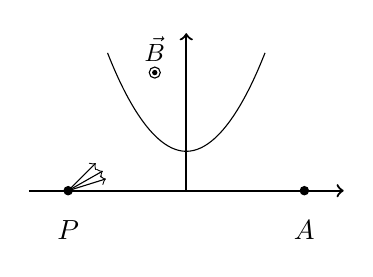
\begin{tikzpicture}
		\draw[thick,->] (-2,0) -- (2,0);
		\draw[thick,->] (0,0) -- (0,2);
		\filldraw[black] (-1.5,0) circle (1.5pt);
		\filldraw[black] (1.5,0) circle (1.5pt);
		\node at (-1.5,-.5) {$P$};
		\node at (1.5,-.5) {$A$};
		\draw[->] (-1.5,0) -- (-1.15,.35);
		\draw[->] (-1.5,0) -- (-1.06,0.25);
		\draw[->] (-1.5,0) -- (-1.02,0.15);
		\draw (0,.5) parabola (1,1.75);
		\draw (0,.5) parabola (-1,1.75);
		\filldraw[black] (-.4,1.5) circle (.75pt);
		\draw (-.4,1.5) circle (2pt);
		\node at (-.4,1.8) {\small $\vec{B}$};
		\end{tikzpicture}\\
	\end{center}
	Ein Strahl positiv geladener Ionen der Ladung $+e$ und der Masse $m$ breitet sich vom Punkt $P$ gleichmäßig in alle Richtungen aus. Dabei wurden die Ionen zuvor mit einer Spannung $U$ beschleunigt.\\
	In der Ebene der Elektroenenausbreitung befindet sich nun ein homogenes Magnetfeld der Stärke $B$, welches senkrecht auf dieser steht. Die Begrenzungslinien des Magnetfeldes sind gerade so, dass die anfangs im Punkt $P$ diviergierenden Ionen im Punkt $A$ wieder fokusiert werden. Wir wollen diese Begrenzungslinien nun näher beschreiben.\\
	Dazu nehmen wir an, dass die Ionenbahn spiegelsymmetrisch zur Mittelsenkrechten auf $\overline{PA}$ ist. Gleichzeitig sollen sowohl $P$ und $A$ nicht im Magnetfeld liegen. 
	\begin{enumerate}[a)]
		\item Berechne den Krümmungsradius einer Ionenbahn in Abhängigkeit von $U$ und $B$, sowie auftretender Konstanten.
		\item Beschreibe charakterstische Eigenschaften der Ionenbahn in diesem System.
		\item Konstruiere die Begrenzungslinien des Magnetfeldes für die Fälle $R<a$, $R=a$ und $R>a$. 	Dabei ist $a = \overline{PA}/2$.
		\item Finde eine Gleichung, die diese Begrenzungslinien beschreibt.
	\end{enumerate}

\end{Exercise}